\documentclass[a4paper]{article} 
\addtolength{\hoffset}{-2.25cm}
\addtolength{\textwidth}{4.5cm}
\addtolength{\voffset}{-3.25cm}
\addtolength{\textheight}{5cm}
\setlength{\parskip}{0pt}
\setlength{\parindent}{0in}

%----------------------------------------------------------------------------------------
%	PACKAGES AND OTHER DOCUMENT CONFIGURATIONS
%----------------------------------------------------------------------------------------

\usepackage{blindtext} % Package to generate dummy text
\usepackage{charter} % Use the Charter font
\usepackage[utf8]{inputenc} % Use UTF-8 encoding
\usepackage{microtype} % Slightly tweak font spacing for aesthetics
\usepackage[ngerman,english]{babel} % Language hyphenation and typographical rules
\usepackage{amsthm, amsmath, amssymb} % Mathematical typesetting
\usepackage{float} % Improved interface for floating objects
\usepackage[final, colorlinks = true, 
            linkcolor = black, 
            citecolor = black]{hyperref} % For hyperlinks in the PDF
\usepackage{graphicx, multicol} % Enhanced support for graphics
\usepackage{xcolor} % Driver-independent color extensions
\usepackage{marvosym, wasysym} % More symbols
\usepackage{rotating} % Rotation tools
\usepackage{censor} % Facilities for controlling restricted text
\usepackage{listings, style/lstlisting} % Environment for non-formatted code, !uses style file!
\usepackage{pseudocode} % Environment for specifying algorithms in a natural way
\usepackage{style/avm} % Environment for f-structures, !uses style file!
\usepackage{booktabs} % Enhances quality of tables
\usepackage{tikz-qtree} % Easy tree drawing tool
\tikzset{every tree node/.style={align=center,anchor=north},
         level distance=2cm} % Configuration for q-trees
\usepackage{style/btree} % Configuration for b-trees and b+-trees, !uses style file!
\usepackage[backend=biber,style=numeric,
            sorting=nyt]{biblatex} % Complete reimplementation of bibliographic facilities
\addbibresource{ecl.bib}
\usepackage{csquotes} % Context sensitive quotation facilities
\usepackage[yyyymmdd]{datetime} % Uses YEAR-MONTH-DAY format for dates
\renewcommand{\dateseparator}{-} % Sets dateseparator to '-'
\usepackage{fancyhdr} % Headers and footers
\pagestyle{fancy} % All pages have headers and footers
\fancyhead{}\renewcommand{\headrulewidth}{0pt} % Blank out the default header
\fancyfoot[L]{} % Custom footer text
\fancyfoot[C]{} % Custom footer text
\fancyfoot[R]{\thepage} % Custom footer text
\newcommand{\note}[1]{\marginpar{\scriptsize \textcolor{red}{#1}}} % Enables comments in red on margin

%----------------------------------------------------------------------------------------

\begin{document}

%-------------------------------
%	TITLE SECTION
%-------------------------------

\fancyhead[C]{}
\hrule \medskip % Upper rule
\begin{minipage}{0.295\textwidth} 
\raggedright
\footnotesize
Akshit Kumar \hfill\\   
EE14B127\hfill\\
\end{minipage}
\begin{minipage}{0.4\textwidth} 
\centering 
\large 
Programming Assignment 2 : Convolutional Neural Networks\\ 
\normalsize 
Deep Learning for Imaging (EE6132)\\ 
\end{minipage}
\begin{minipage}{0.295\textwidth} 
\raggedleft
\today\hfill\\
\end{minipage}
\medskip\hrule 
\bigskip

%-------------------------------
%	CONTENTS
%-------------------------------
\tableofcontents
\section{MNIST Classification Using CNN}
In this section, we consider three architectures of the CNN which are presented below:
\begin{itemize}
\item Model 1 - 1 Convolutional Layer 
\item Model 2 - 2 Convolutional Layer 
\item Model 3 - 2 Convolutional Layer + 1 hidden fully connected layer 
\end{itemize}
The fully description of the architecture is given in each corresponding section.
\subsection{Model 1 - 1 Convolutional Layer}
\subsubsection{Detailed Architecture}
The 1 Convolutional Layer CNN has the following architecture:
\begin{itemize}
\item Input
\item Conv Layer
	\begin{itemize}
	\item Number of Filters = 32
	\item Filter Size - $3 \times 3$
    \item Stride = 1
    \item Zero Padding of 1
	\end{itemize}
\item Max Pool Layer
\begin{itemize}
\item $2\times2$ Max Pooling
\item Stride = 2
\end{itemize}
\item Fully Connected (10 Outputs)
\item Softmax Classifer
\end{itemize}
\subsubsection{Plot of Randomly Selected Test Images}
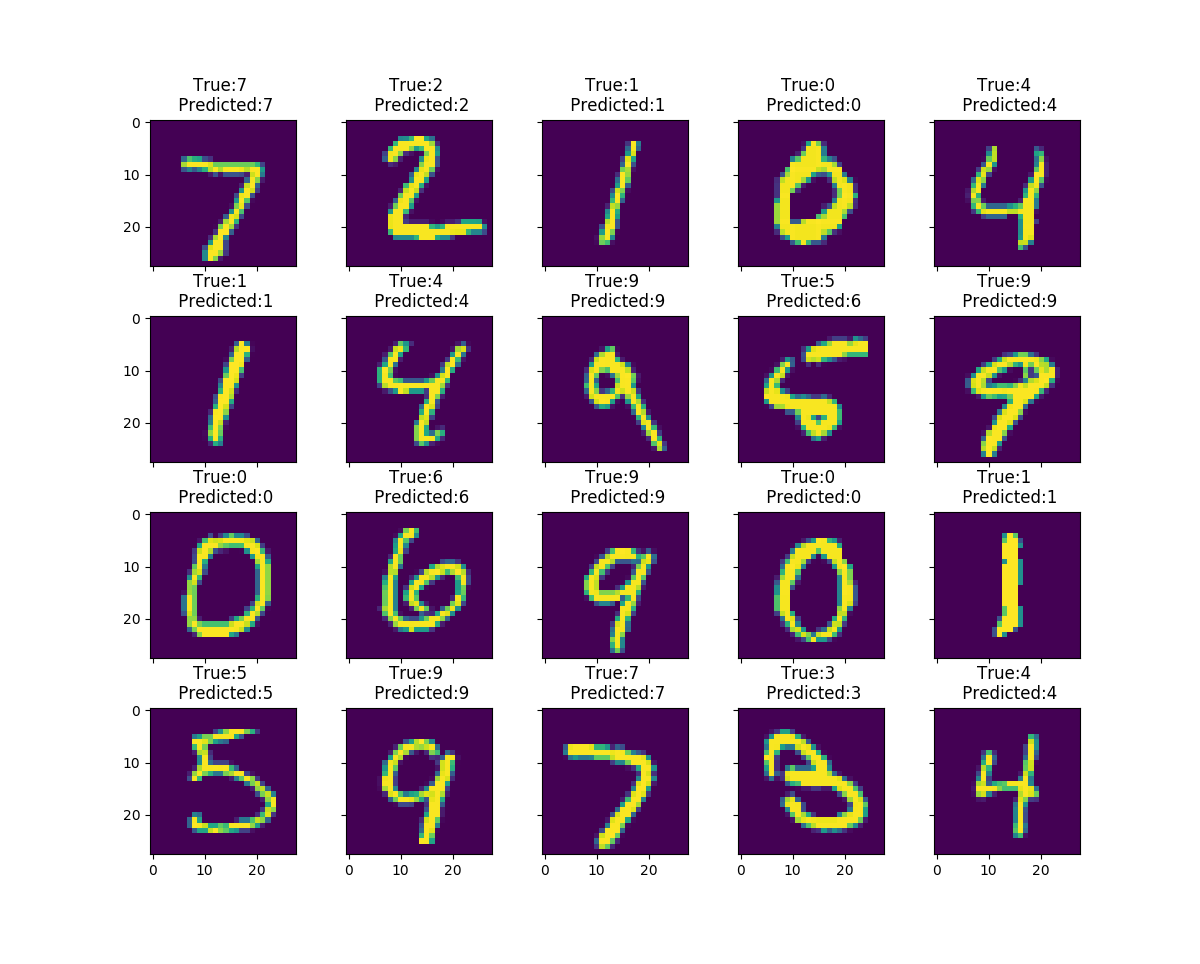
\includegraphics[scale=0.55]{prediction_model1}

\subsection{Model 2 - 2 Convolutional Layer}
\subsubsection{Detailed Architecture}
The 2 Convolutional Layer CNN has the following architecture:
\begin{itemize}
\item Input
\item Conv Layer 1
	\begin{itemize}
	\item Number of Filters = 32
	\item Filter Size - $3 \times 3$
    \item Stride = 1
    \item Zero Padding of 1
	\end{itemize}
\item Max Pool Layer 1
\begin{itemize}
\item $2\times2$ Max Pooling
\item Stride = 2
\end{itemize}
\item Conv Layer 2
	\begin{itemize}
	\item Number of Filters = 32
	\item Filter Size - $3 \times 3$
    \item Stride = 1
    \item Zero Padding of 1
	\end{itemize}
\item Max Pool Layer 2
\begin{itemize}
\item $2\times2$ Max Pooling
\item Stride = 2
\end{itemize}
\item Fully Connected (10 Outputs)
\item Softmax Classifer
\end{itemize}
\subsubsection{Plot of Randomly Selected Test Images}
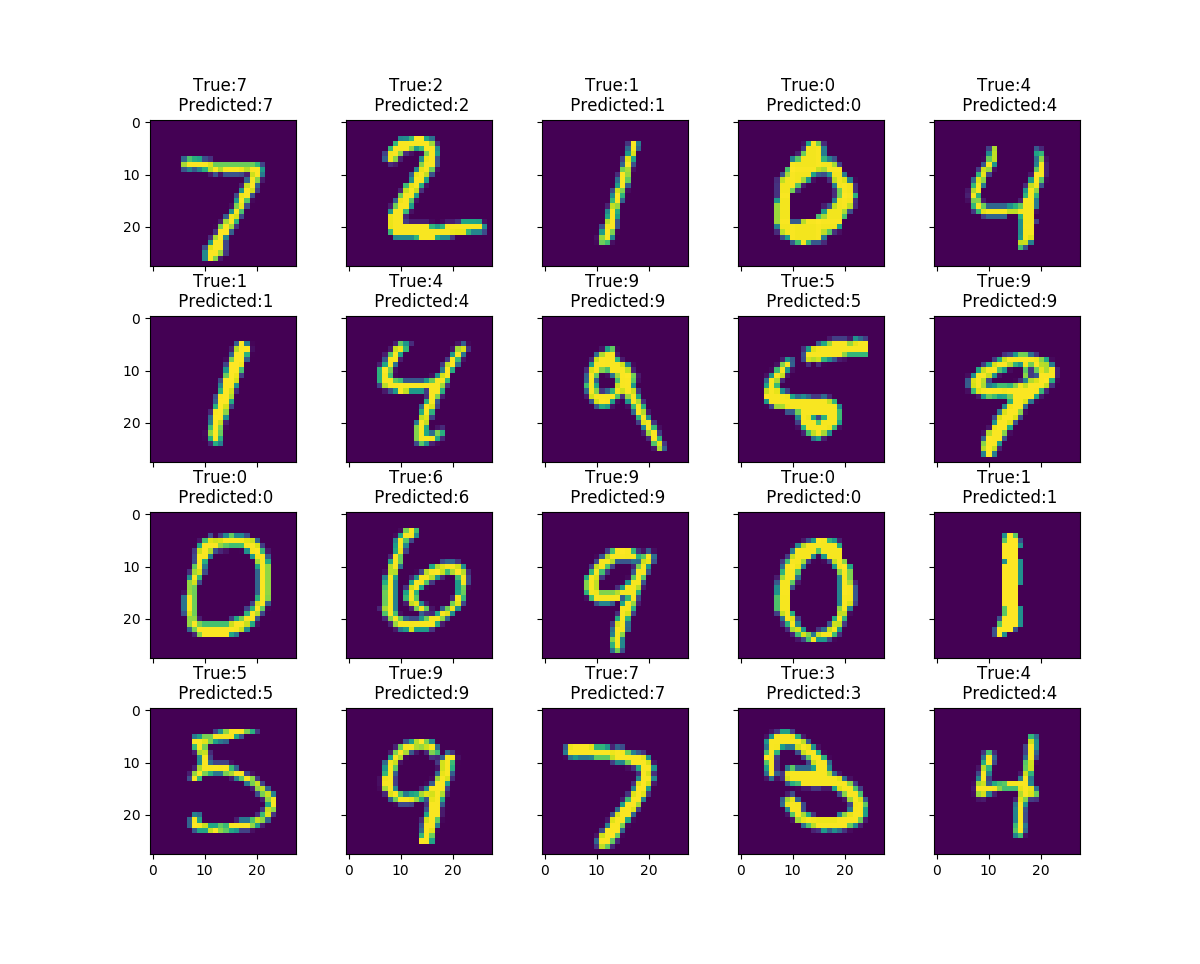
\includegraphics[scale=0.55]{prediction_model2}

\subsection{Model 3 - 2 Convolutional Layer + 1 hidden fully connected layer }
\subsubsection{Detailed Architecture}
The 2 Convolutional Layer + 1 hidden fully connected layer  CNN has the following architecture:
\begin{itemize}
\item Input
\item Conv Layer 1
	\begin{itemize}
	\item Number of Filters = 32
	\item Filter Size - $3 \times 3$
    \item Stride = 1
    \item Zero Padding of 1
	\end{itemize}
\item Max Pool Layer 1
\begin{itemize}
\item $2\times2$ Max Pooling
\item Stride = 2
\end{itemize}
\item Conv Layer 2
	\begin{itemize}
	\item Number of Filters = 32
	\item Filter Size - $3 \times 3$
    \item Stride = 1
    \item Zero Padding of 1
	\end{itemize}
\item Max Pool Layer 2
\begin{itemize}
\item $2\times2$ Max Pooling
\item Stride = 2
\end{itemize}
\item Fully Connected (500 Outputs)
\item Fully Connected (10 Outputs)
\item Softmax Classifer
\end{itemize}
\subsubsection{Plot of Randomly Selected Test Images}
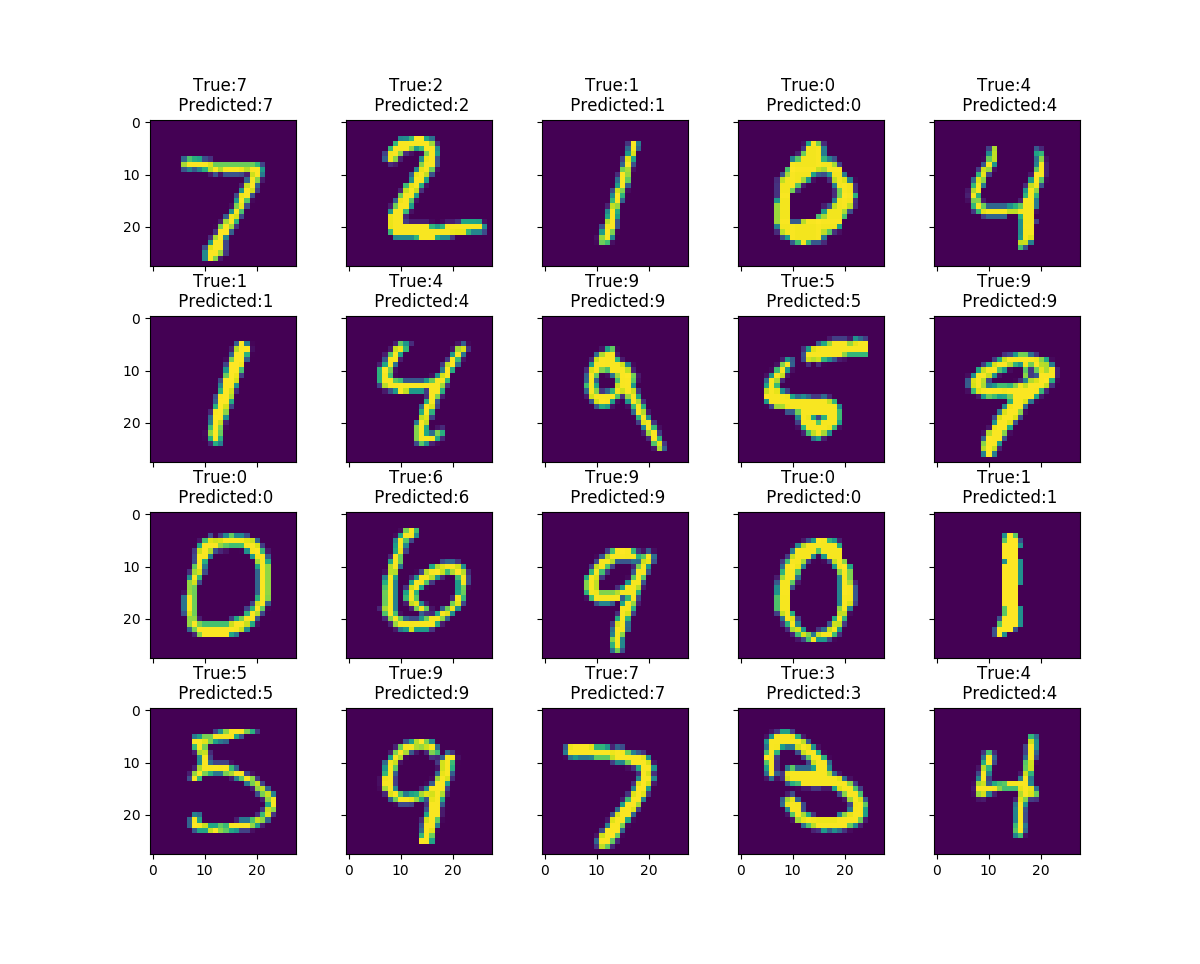
\includegraphics[scale=0.55]{prediction_model3}

\subsection{Comparison of the three models}
The three models are compared on the following three metrics :
\begin{itemize}
\item Training Loss Plot
\item Validation Loss Plot
\item Test Accuracy 
\end{itemize}
\subsubsection{Training Loss Plot}
\begin{center}
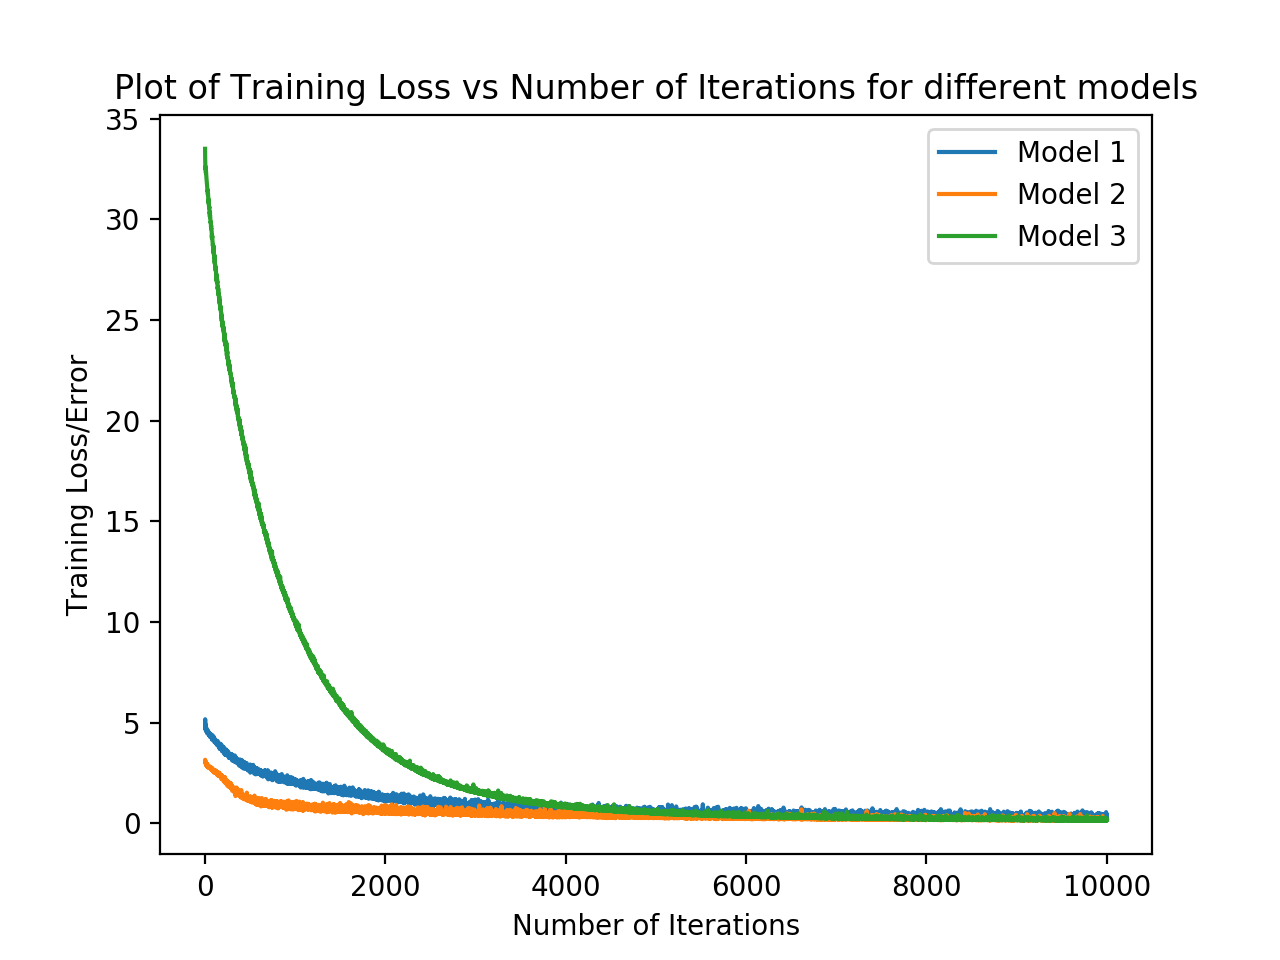
\includegraphics[scale=.6]{training_loss_q1}
\end{center}
\subsubsection{Validation Loss Plot}
\begin{center}
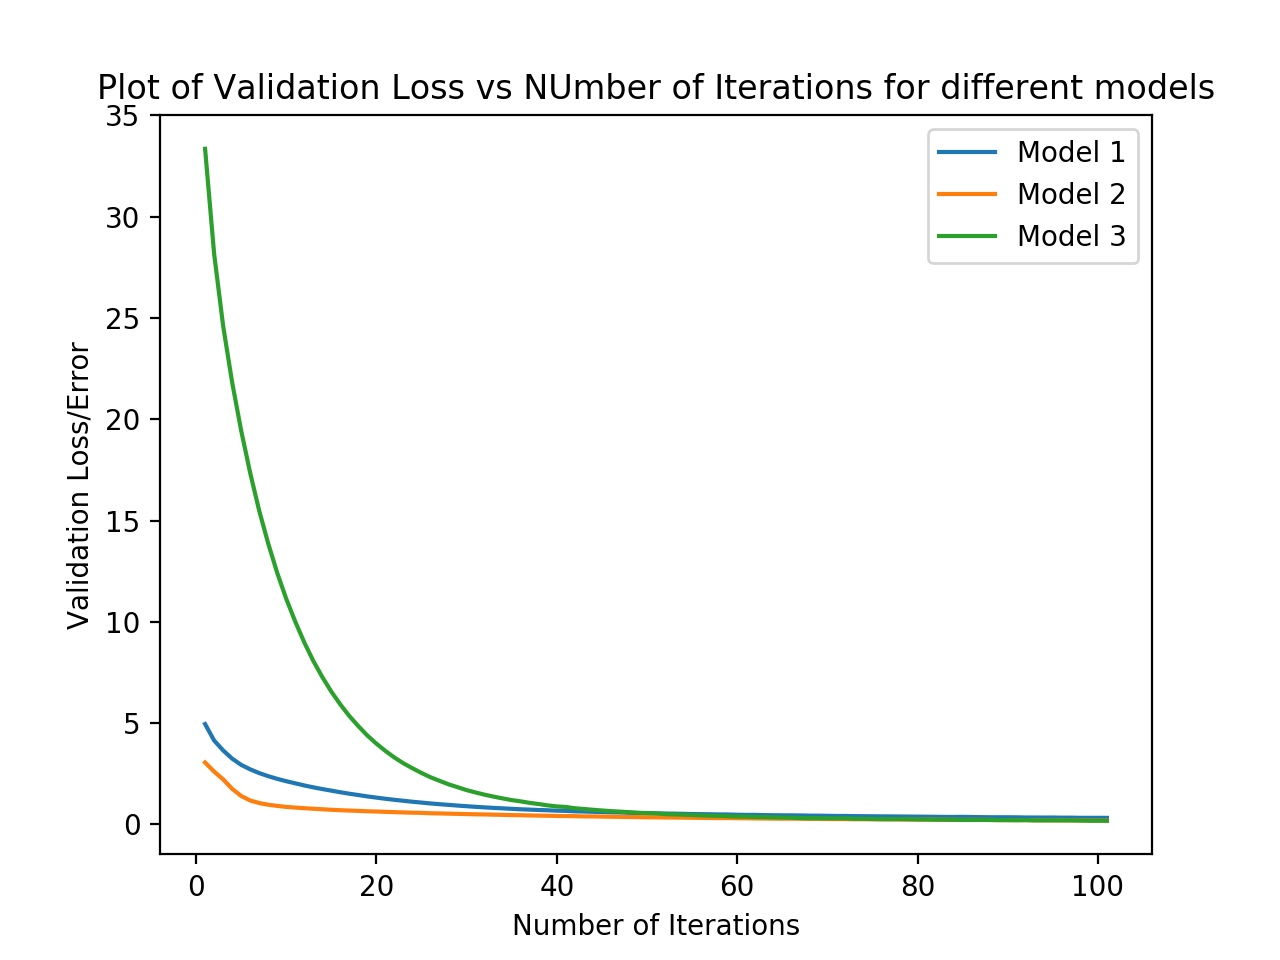
\includegraphics[scale=.6]{validation_loss_q1}
\end{center}
Note that since the validation loss plot is coming down with the increasing number of iterations, we can conclude that none of the models are over-fitting and regularization seems to be working. Also, note that even though it may not be very apparent from the graph, but Model 3 gives the least validation loss/error after 10000 iterations of training.

\subsubsection{Test Accuracy}
\begin{center}
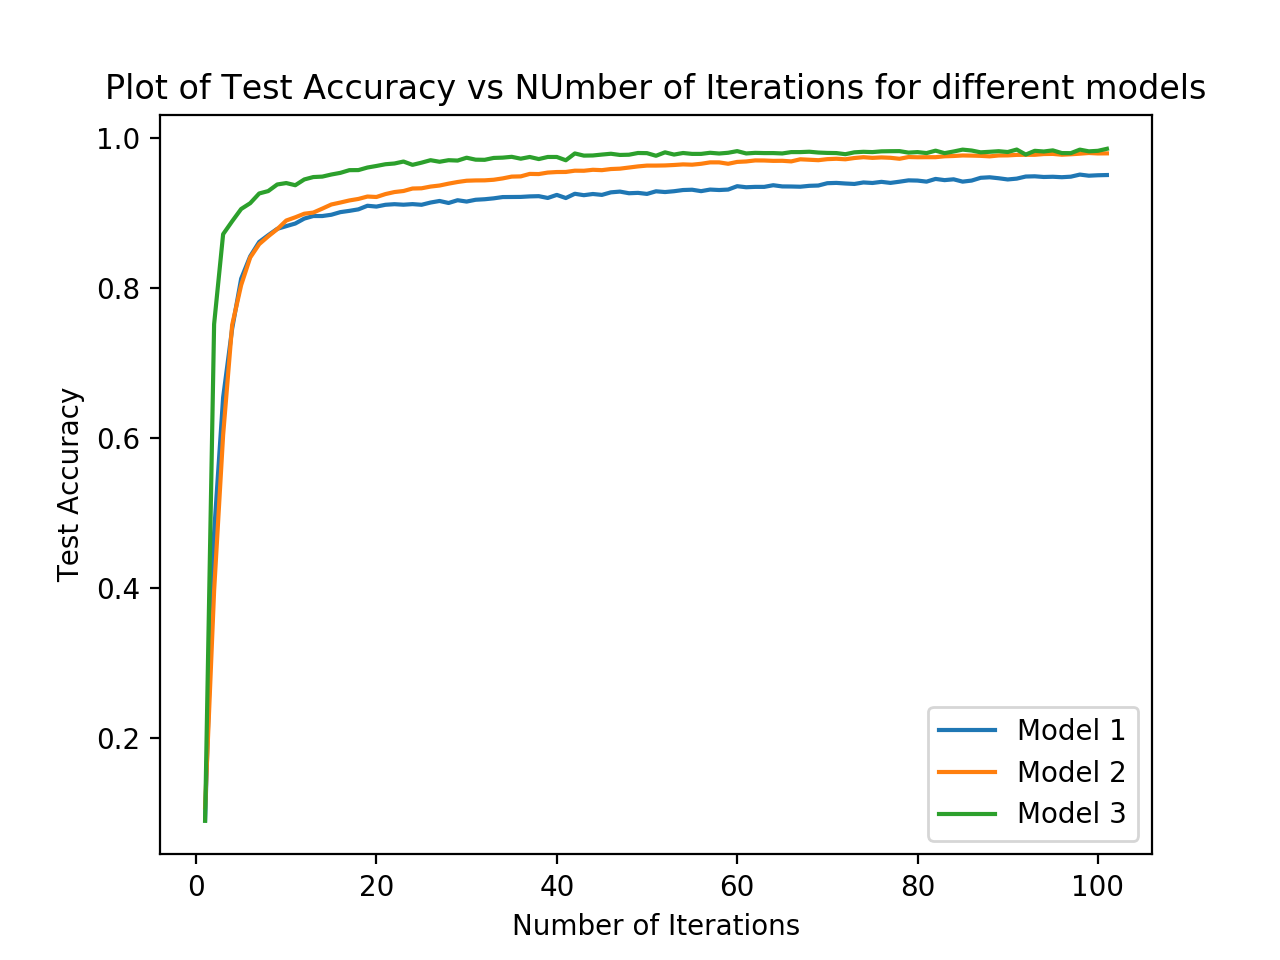
\includegraphics[scale=.6]{test_accuracy_q1}
\end{center}

\begin{center}
\begin{tabular}{|c|c|}
\hline
Model & Test Accuracy \\
\hline
Model 1 - 1 Convolutional Layer & 95.06\%  \\
\hline
Model 2 - 2 Convolutional Layer & 97.96\%  \\
\hline
Model 3 - 2 Convolutional Layer + 1 Hidden Layer & 98.5\%  \\
\hline
\end{tabular}
\end{center}
We can clearly see that Model 3 outperforms the other models in terms of \textbf{Test Accuracy} and hence is the best model learnt. We make use of this learnt model in our future experimentation.

\section{Generating Adversarial Examples}
\subsection{Learning Curves}
Presented below are the learning curves for generating the noise masks for each of the classes from 0 to 9. 
\subsubsection{Plot of Training Loss for all 10 classes}
\begin{center}
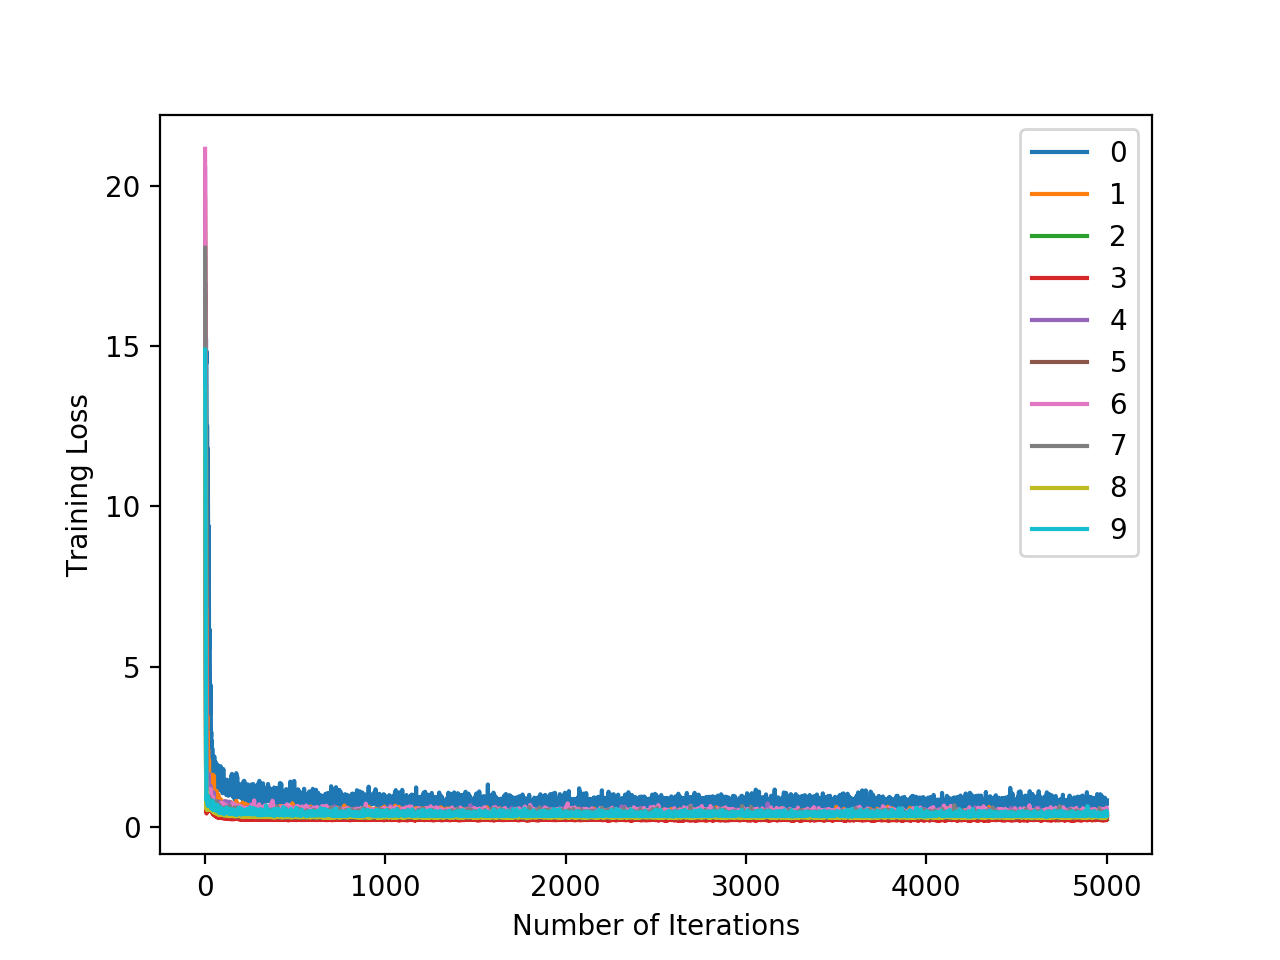
\includegraphics[scale=0.8]{training_loss_q2}
\end{center}
\subsubsection{Plot of Validation Loss for all 10 classes}
\begin{center}
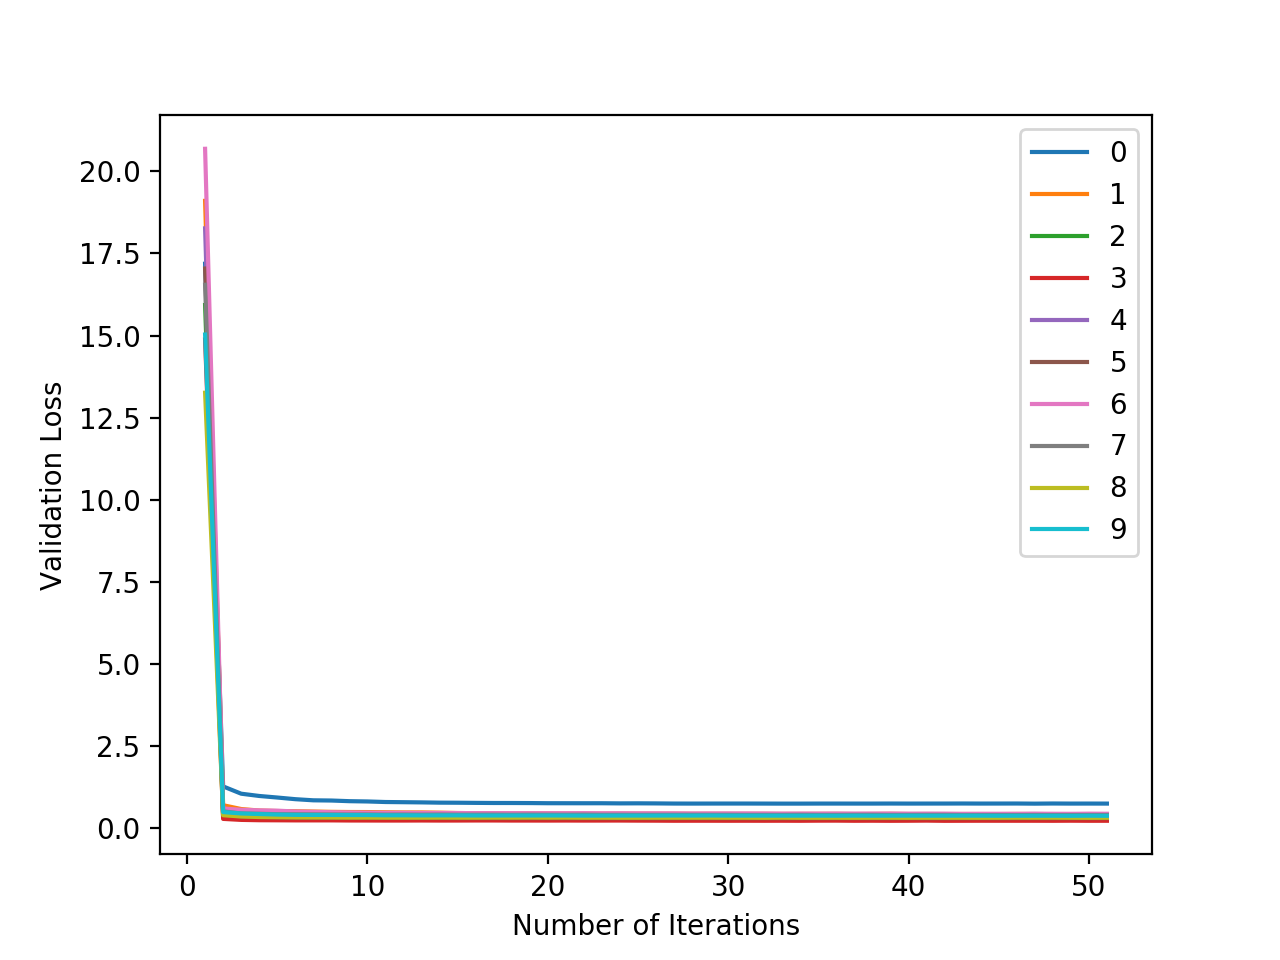
\includegraphics[scale=0.8]{validation_loss_q2}
\end{center}
\subsubsection{Plot of Test Accuracy for all 10 classes}
\begin{center}
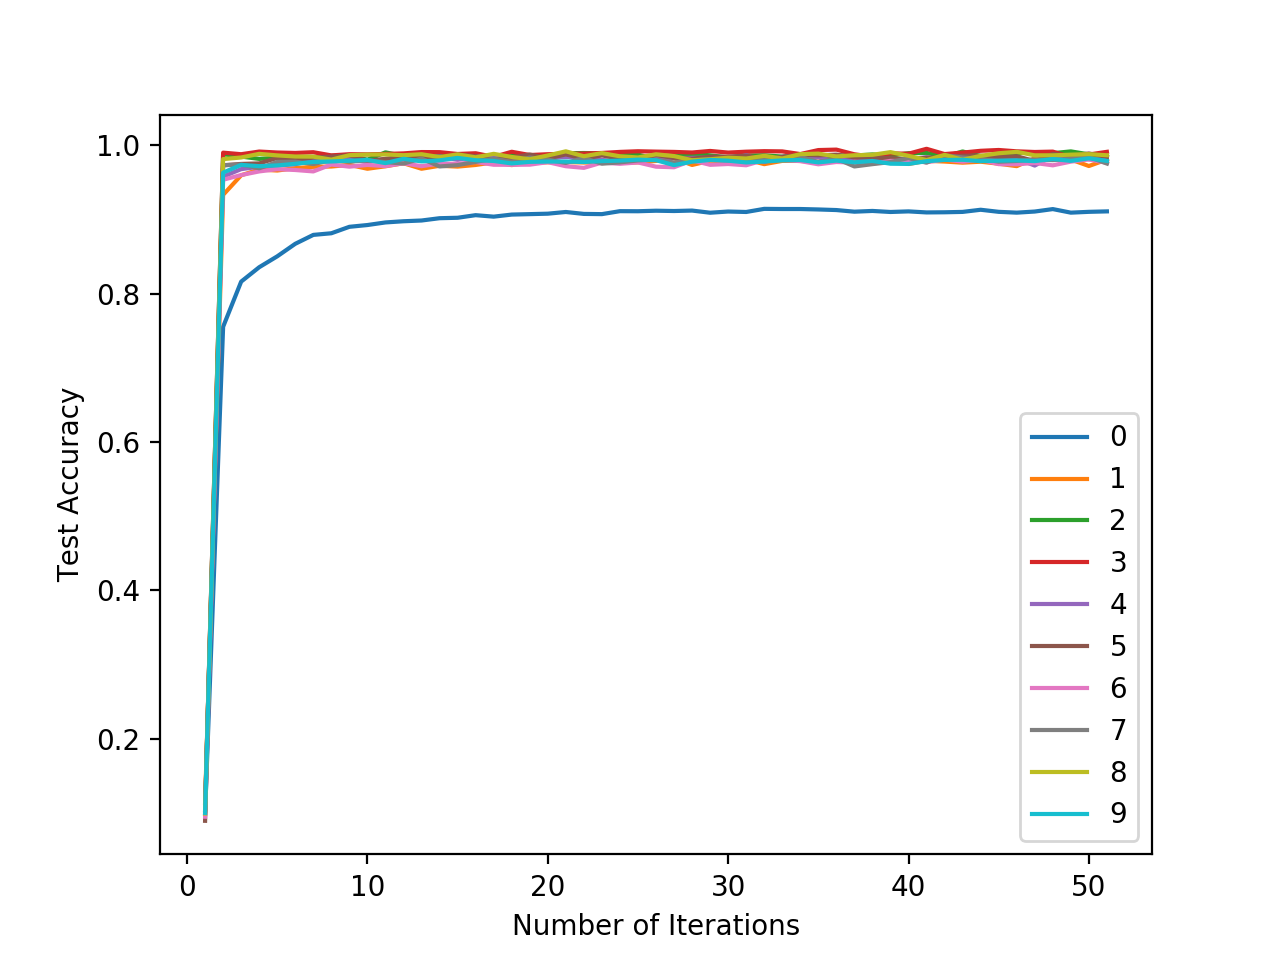
\includegraphics[scale=0.8]{test_accuracy_q2}
\end{center}


\subsection{Plot of All Noise Patterns}
\begin{center}
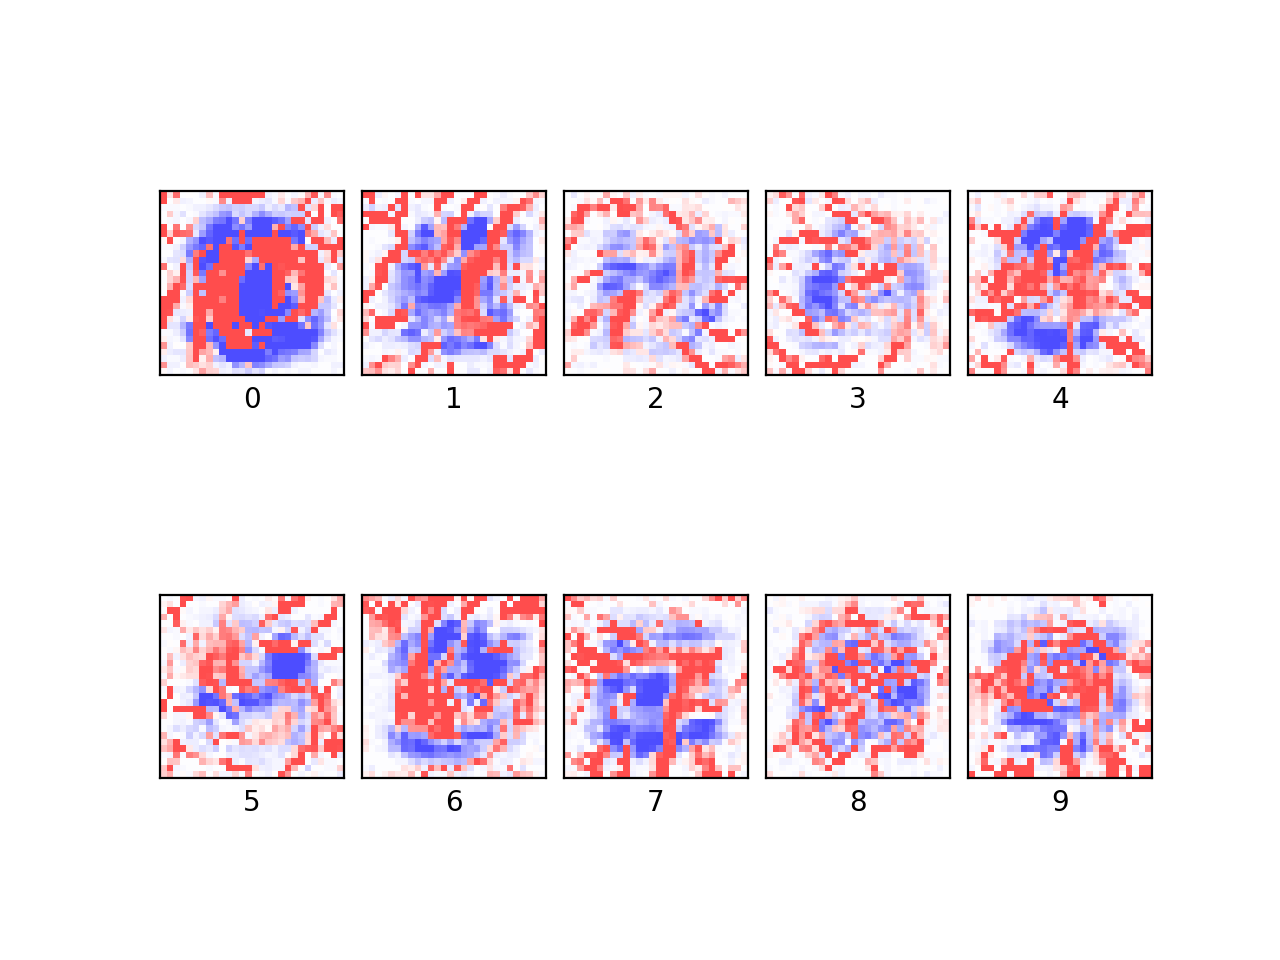
\includegraphics[scale=1]{all_noise}
\end{center}

\subsection{Examples Showing Misclassification Due to Addition of Noise}
\subsubsection{Misclassification with Class 0 Noise}
\begin{center}
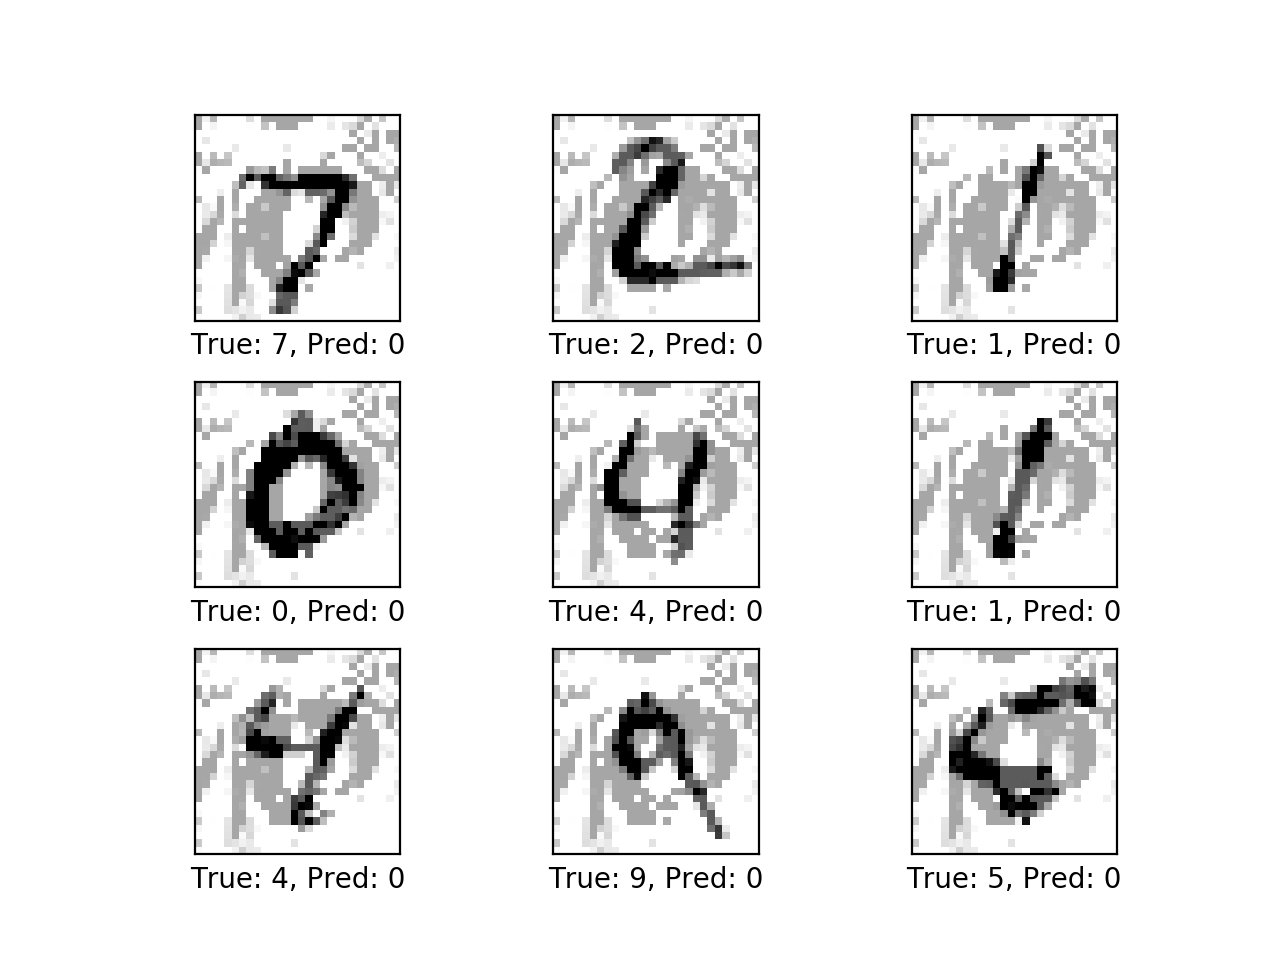
\includegraphics[scale=0.8]{0_noise}
\end{center}

\subsubsection{Misclassification with Class 1 Noise}
\begin{center}
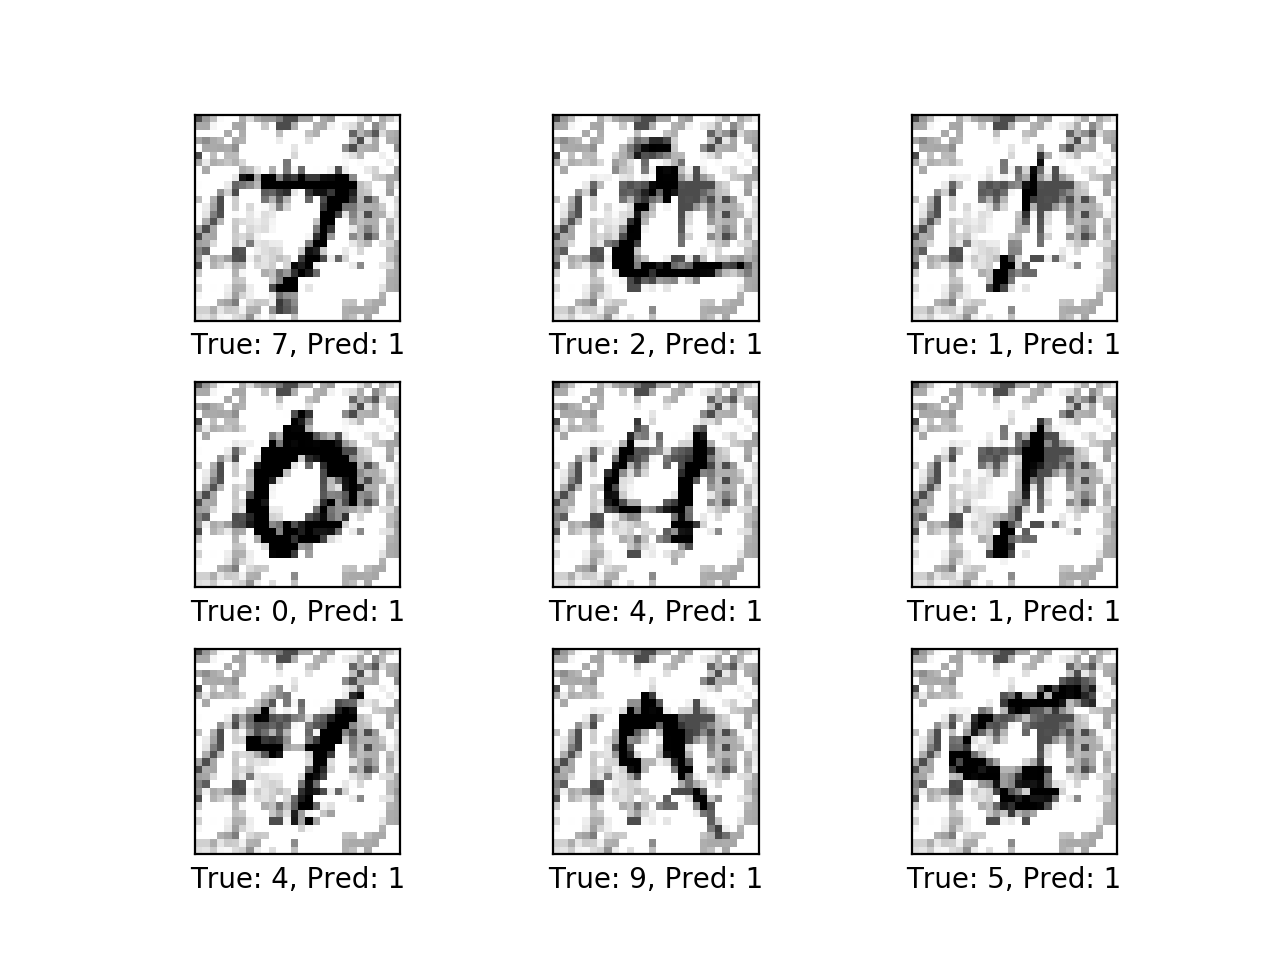
\includegraphics[scale=0.8]{1_noise}
\end{center}

\subsubsection{Misclassification with Class 2 Noise}
\begin{center}
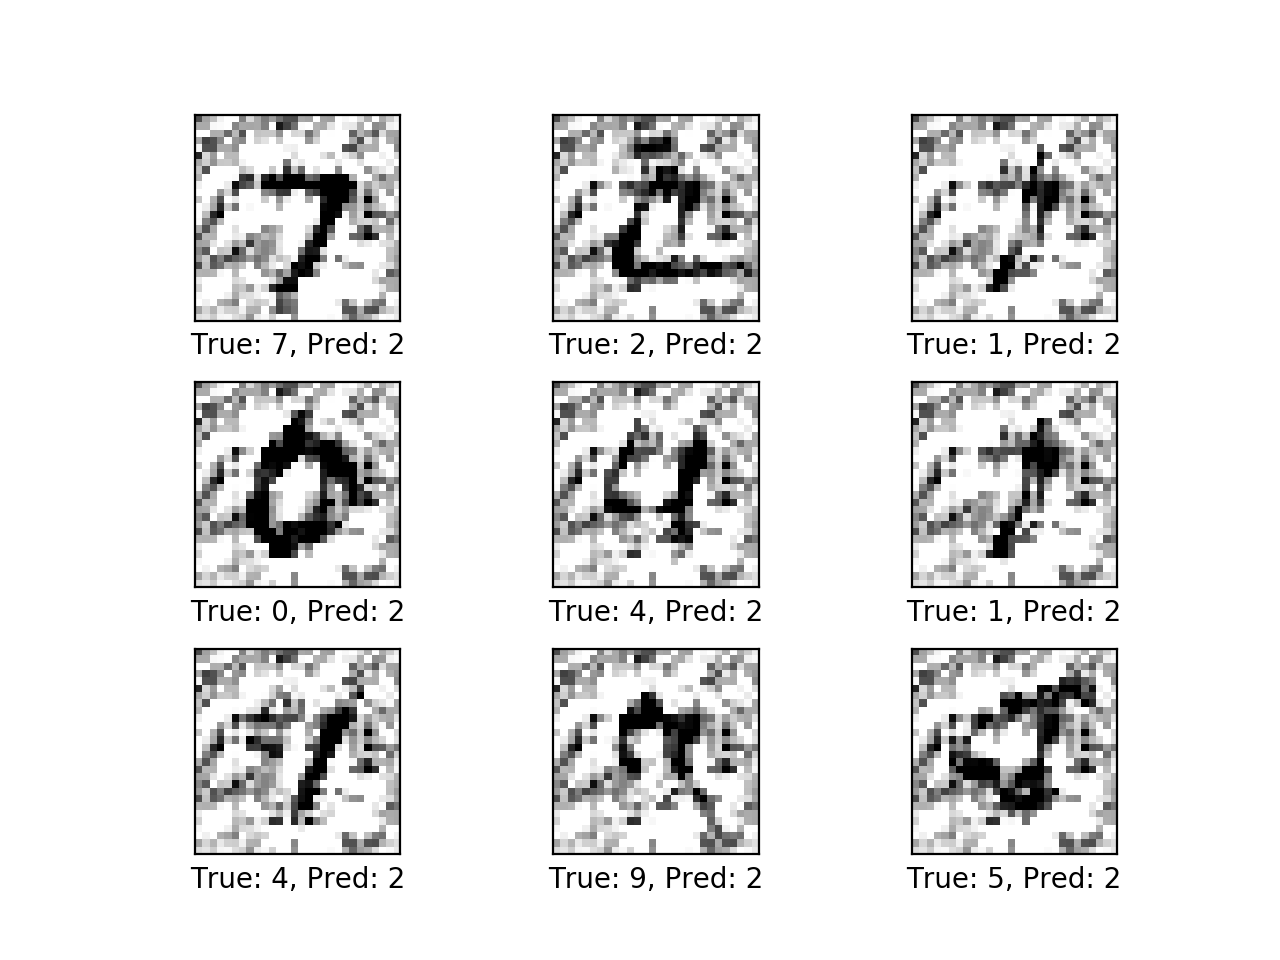
\includegraphics[scale=0.8]{2_noise}
\end{center}

\subsubsection{Misclassification with Class 3 Noise}
\begin{center}
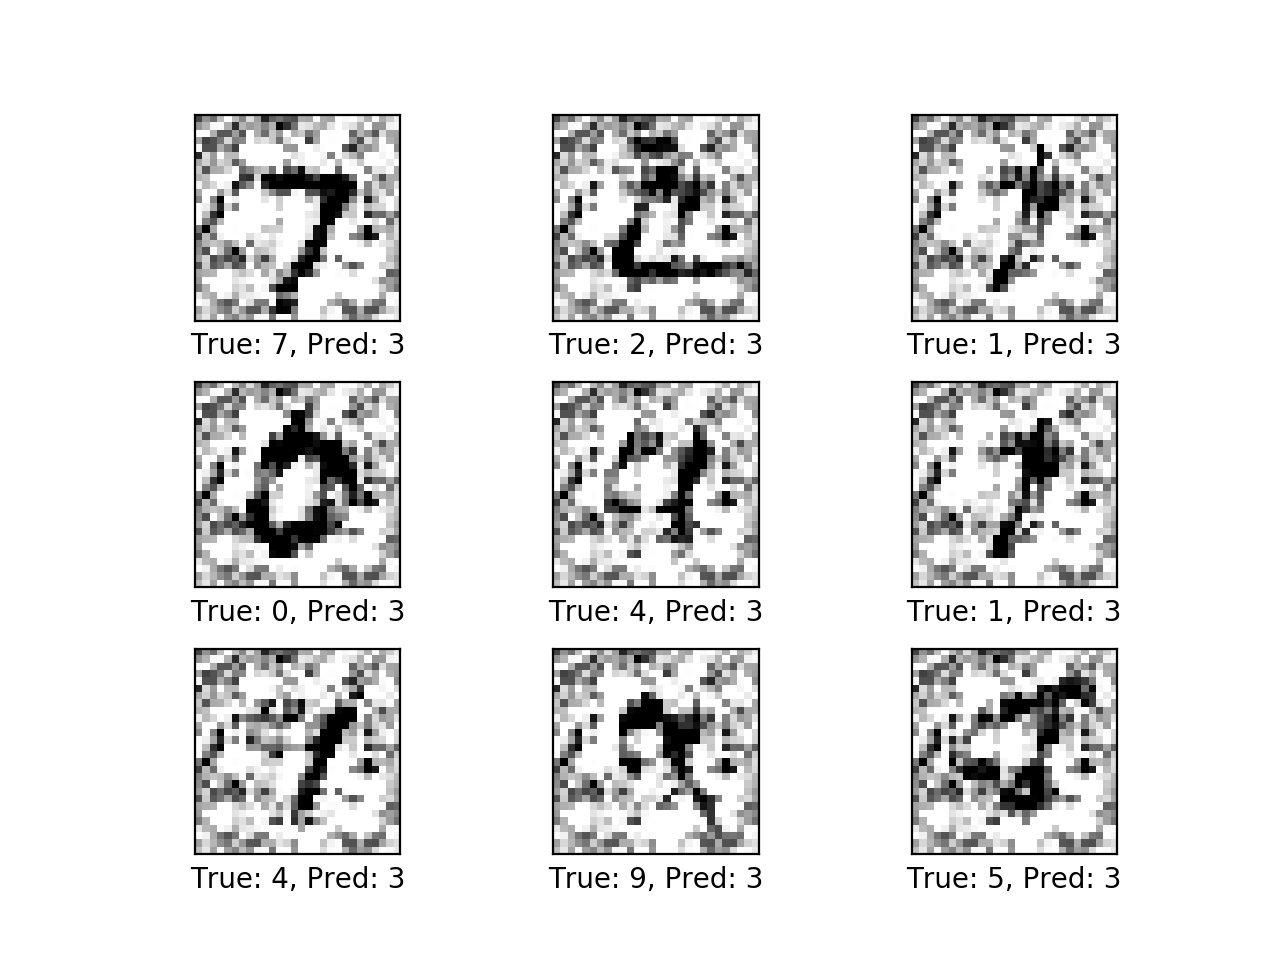
\includegraphics[scale=0.8]{3_noise}
\end{center}

\subsubsection{Misclassification with Class 4 Noise}
\begin{center}
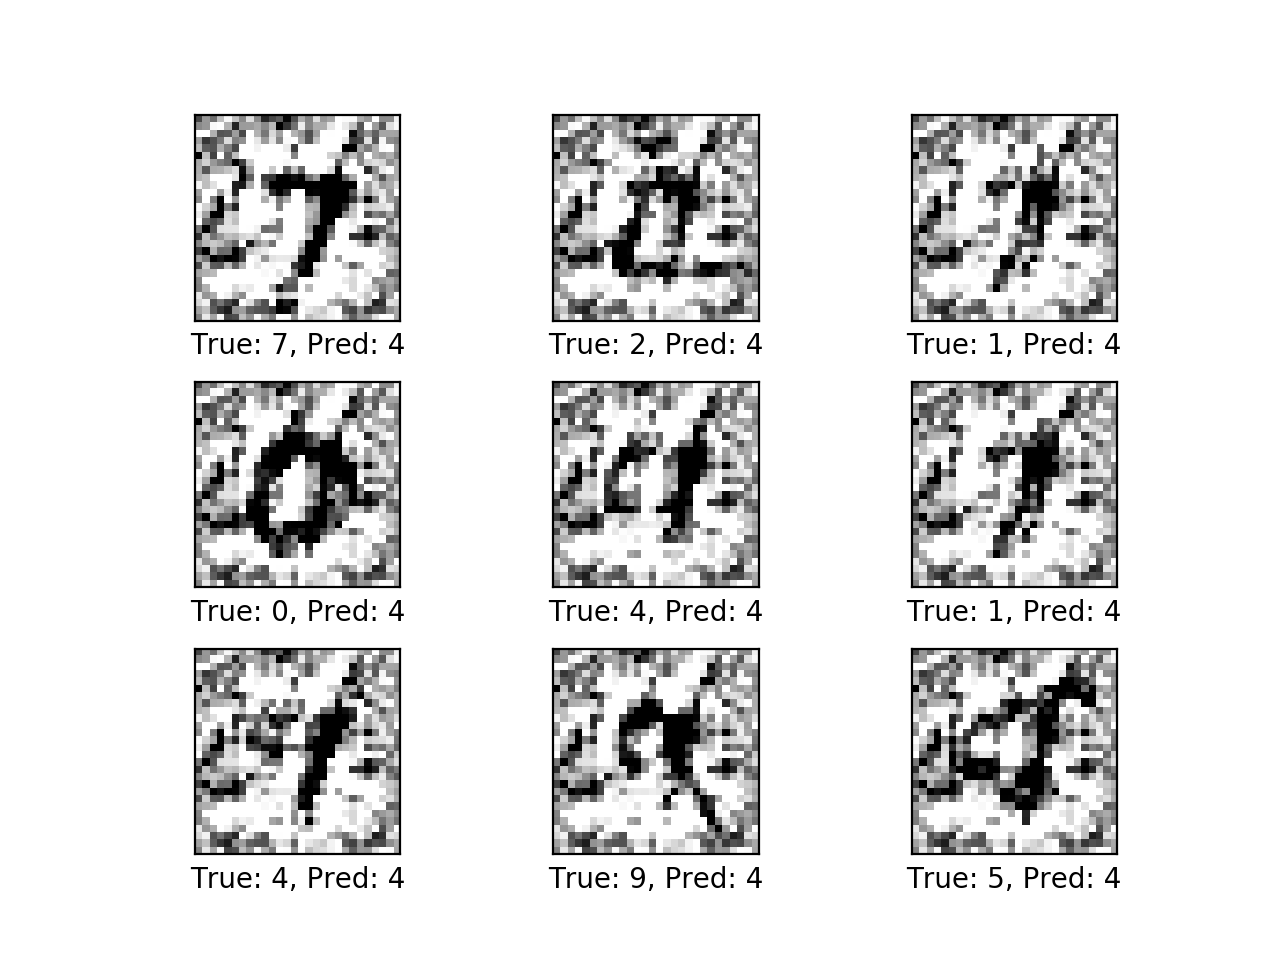
\includegraphics[scale=0.8]{4_noise}
\end{center}

\subsubsection{Misclassification with Class 5 Noise}
\begin{center}
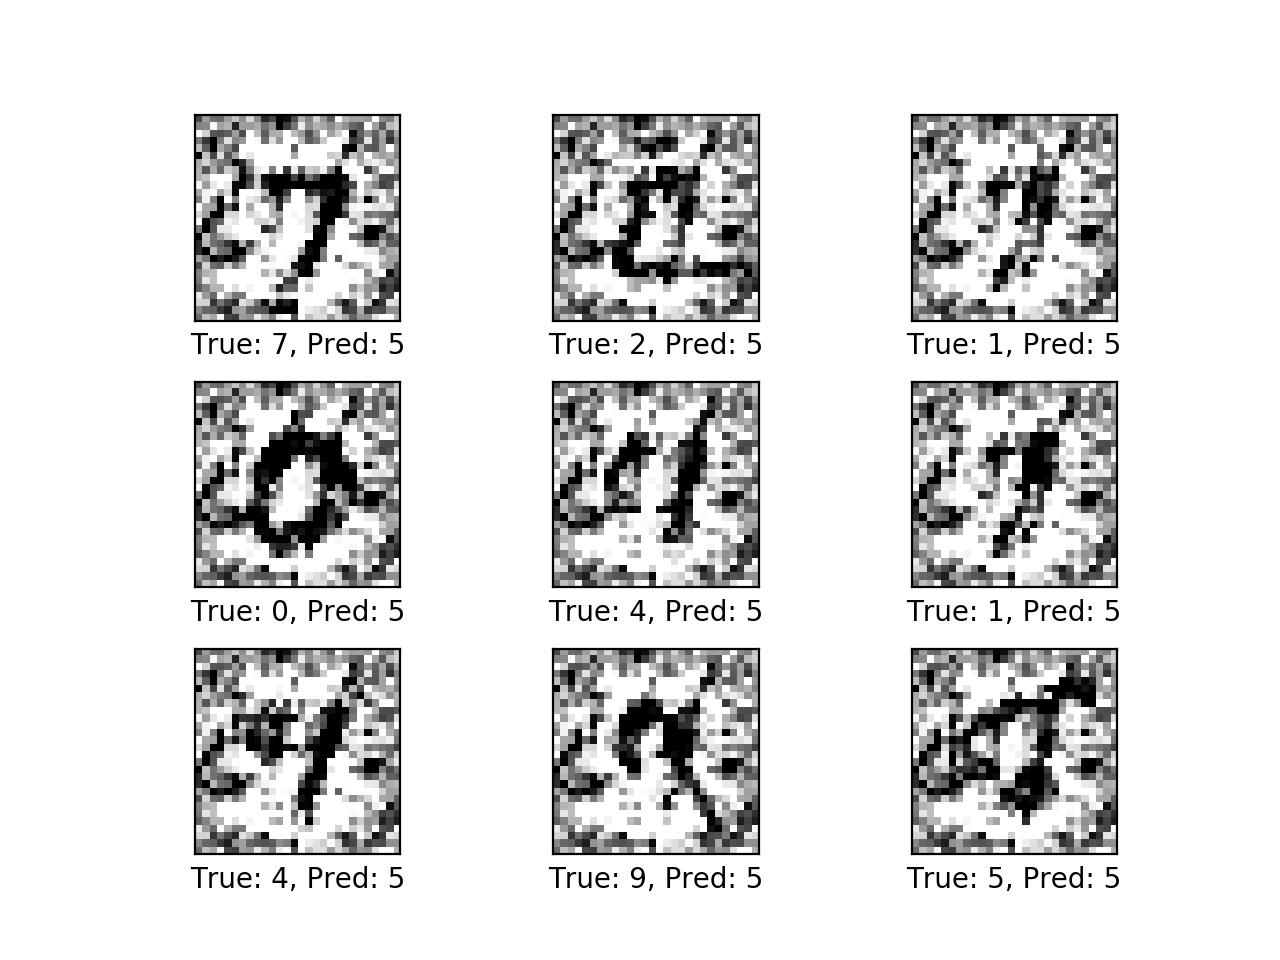
\includegraphics[scale=0.8]{5_noise}
\end{center}

\subsubsection{Misclassification with Class 6 Noise}
\begin{center}
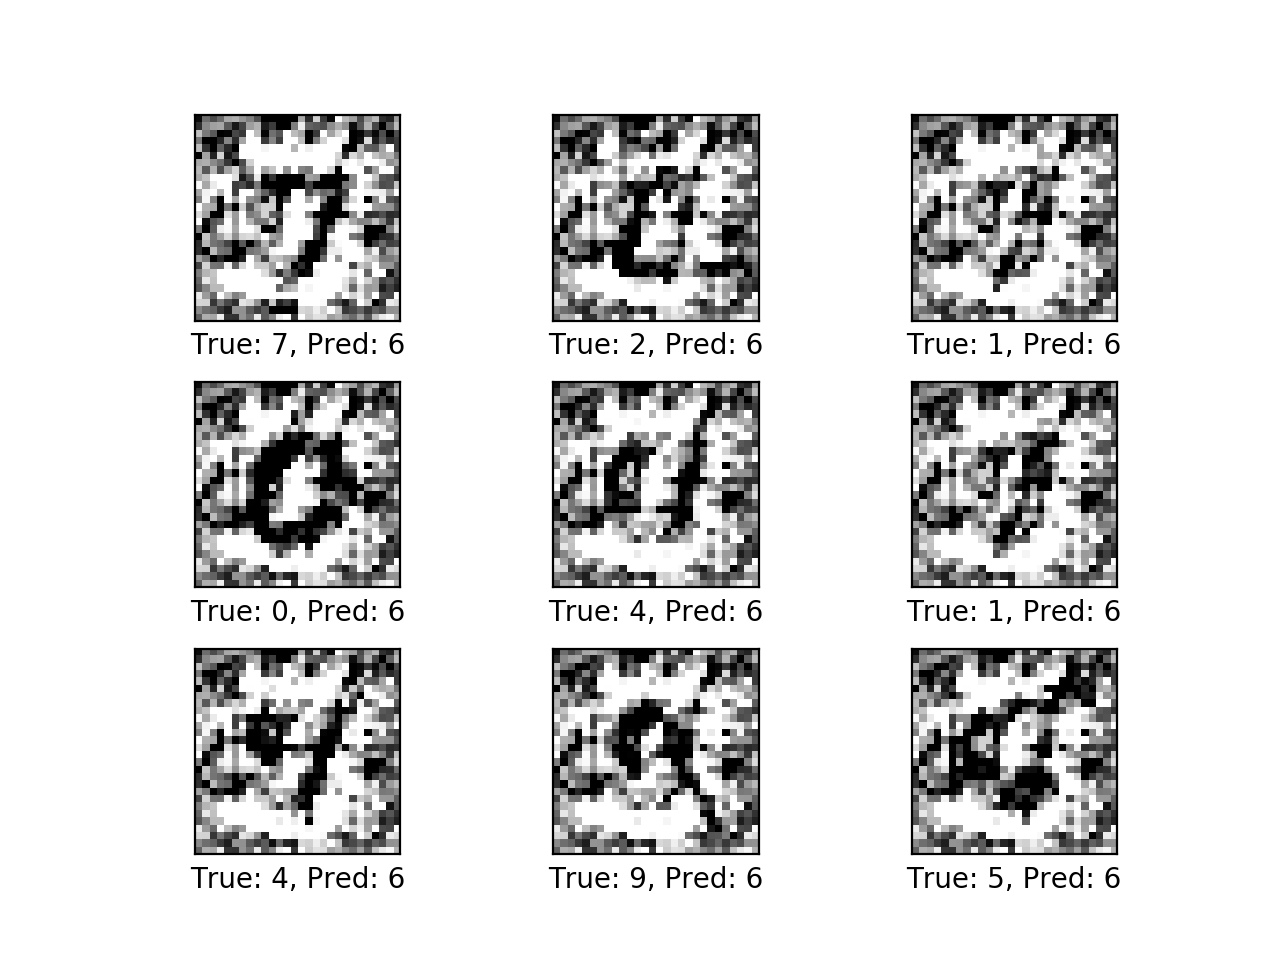
\includegraphics[scale=0.8]{6_noise}
\end{center}

\subsubsection{Misclassification with Class 7 Noise}
\begin{center}
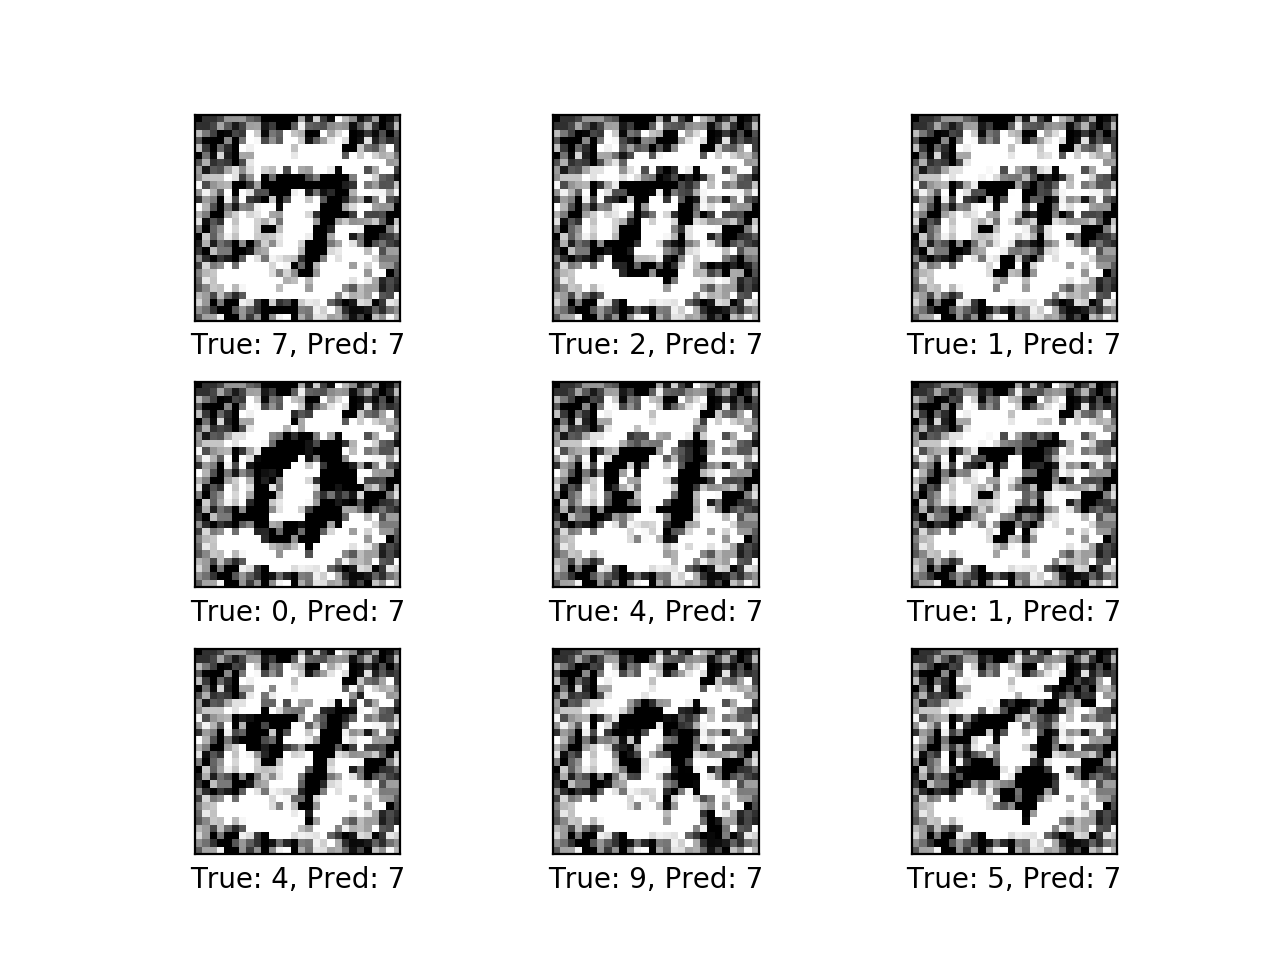
\includegraphics[scale=0.8]{7_noise}
\end{center}

\subsubsection{Misclassification with Class 8 Noise}
\begin{center}
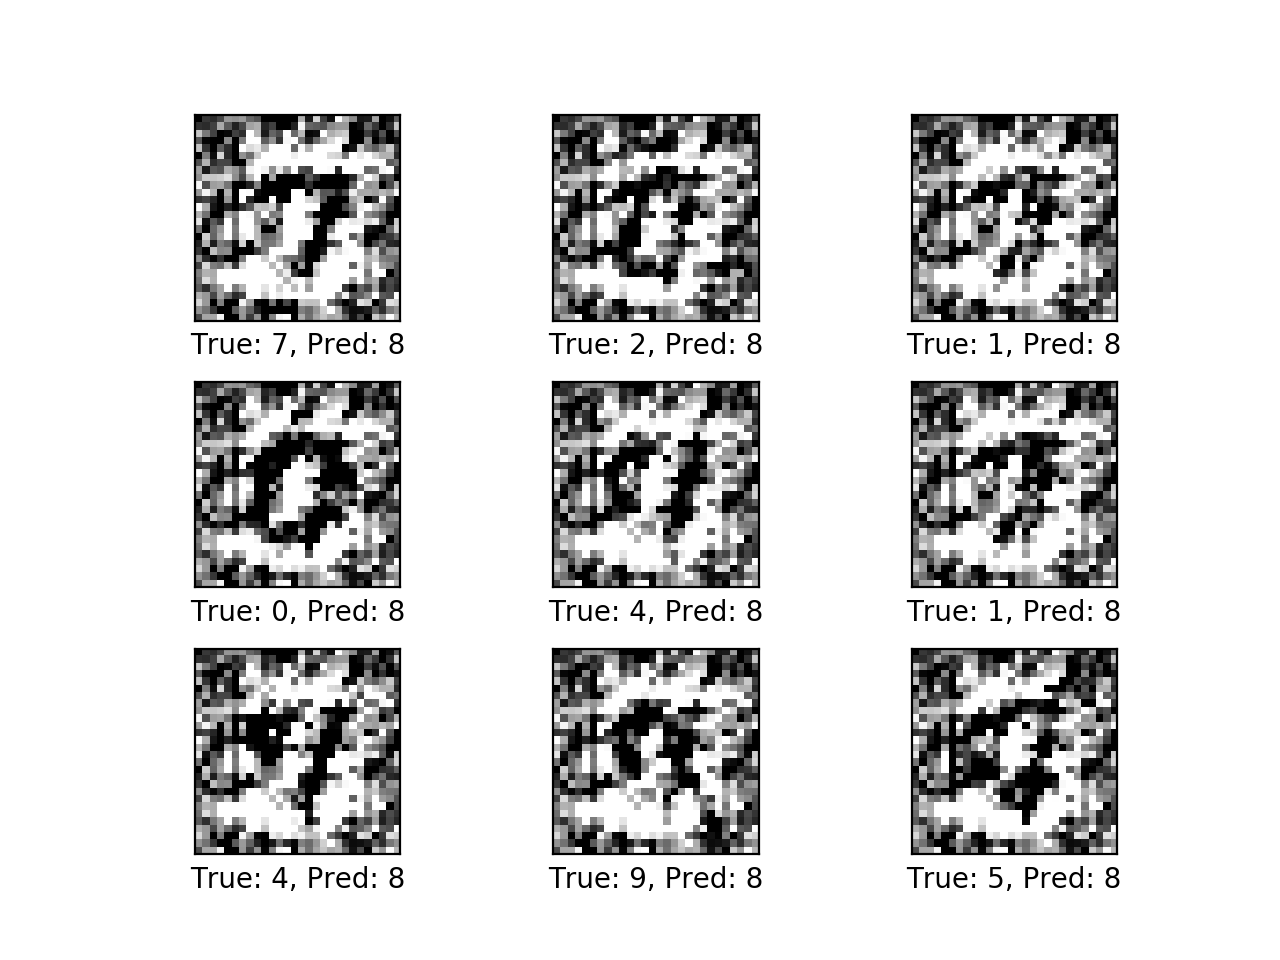
\includegraphics[scale=0.8]{8_noise}
\end{center}

\subsubsection{Misclassification with Class 9 Noise}
\begin{center}
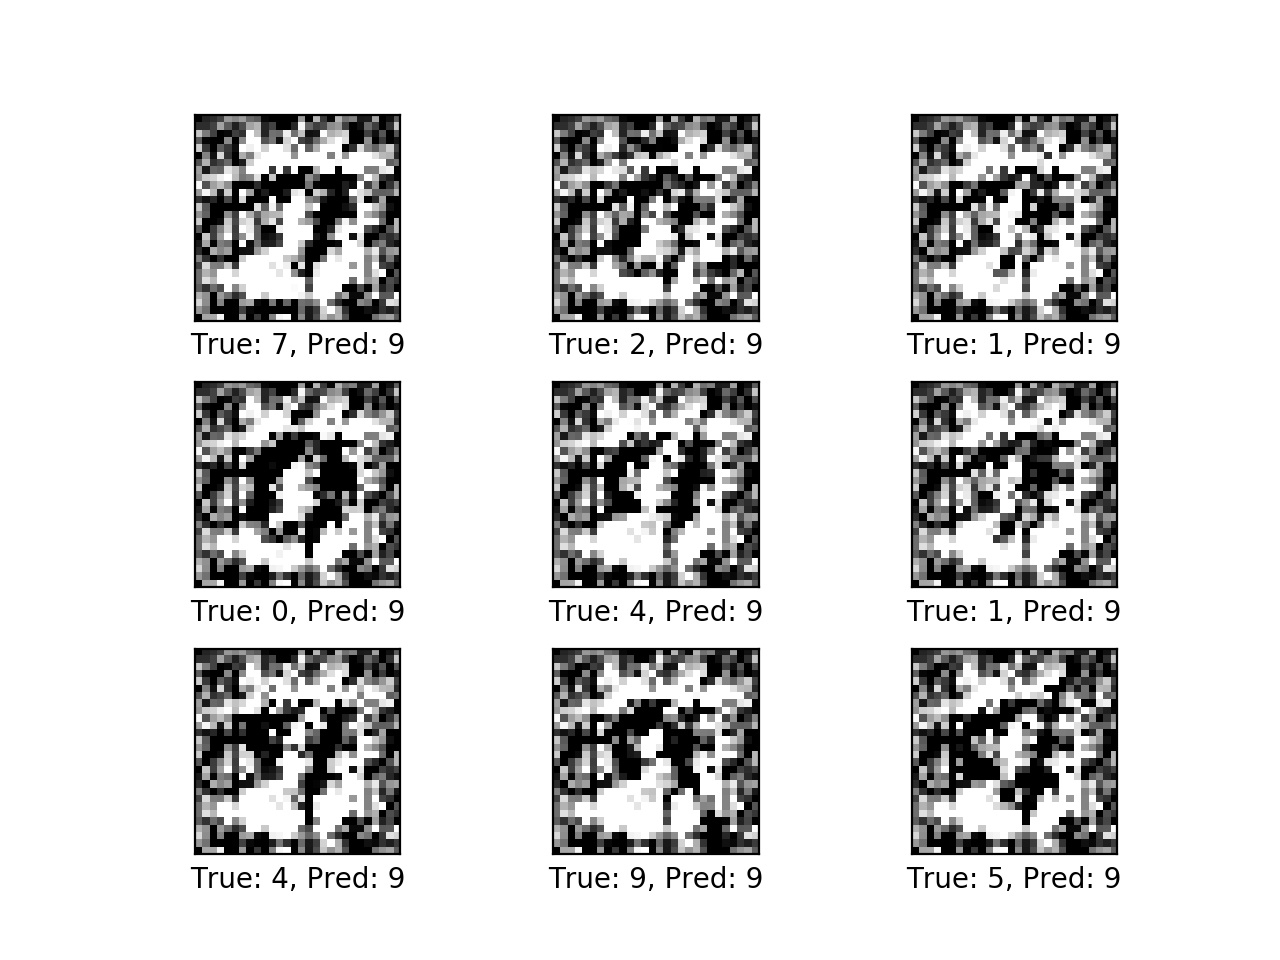
\includegraphics[scale=0.8]{9_noise}
\end{center}

\section{Visualizing the CNN}
\subsection{Plot of $x_{init}$ for 10 Output Neurons}
\begin{center}
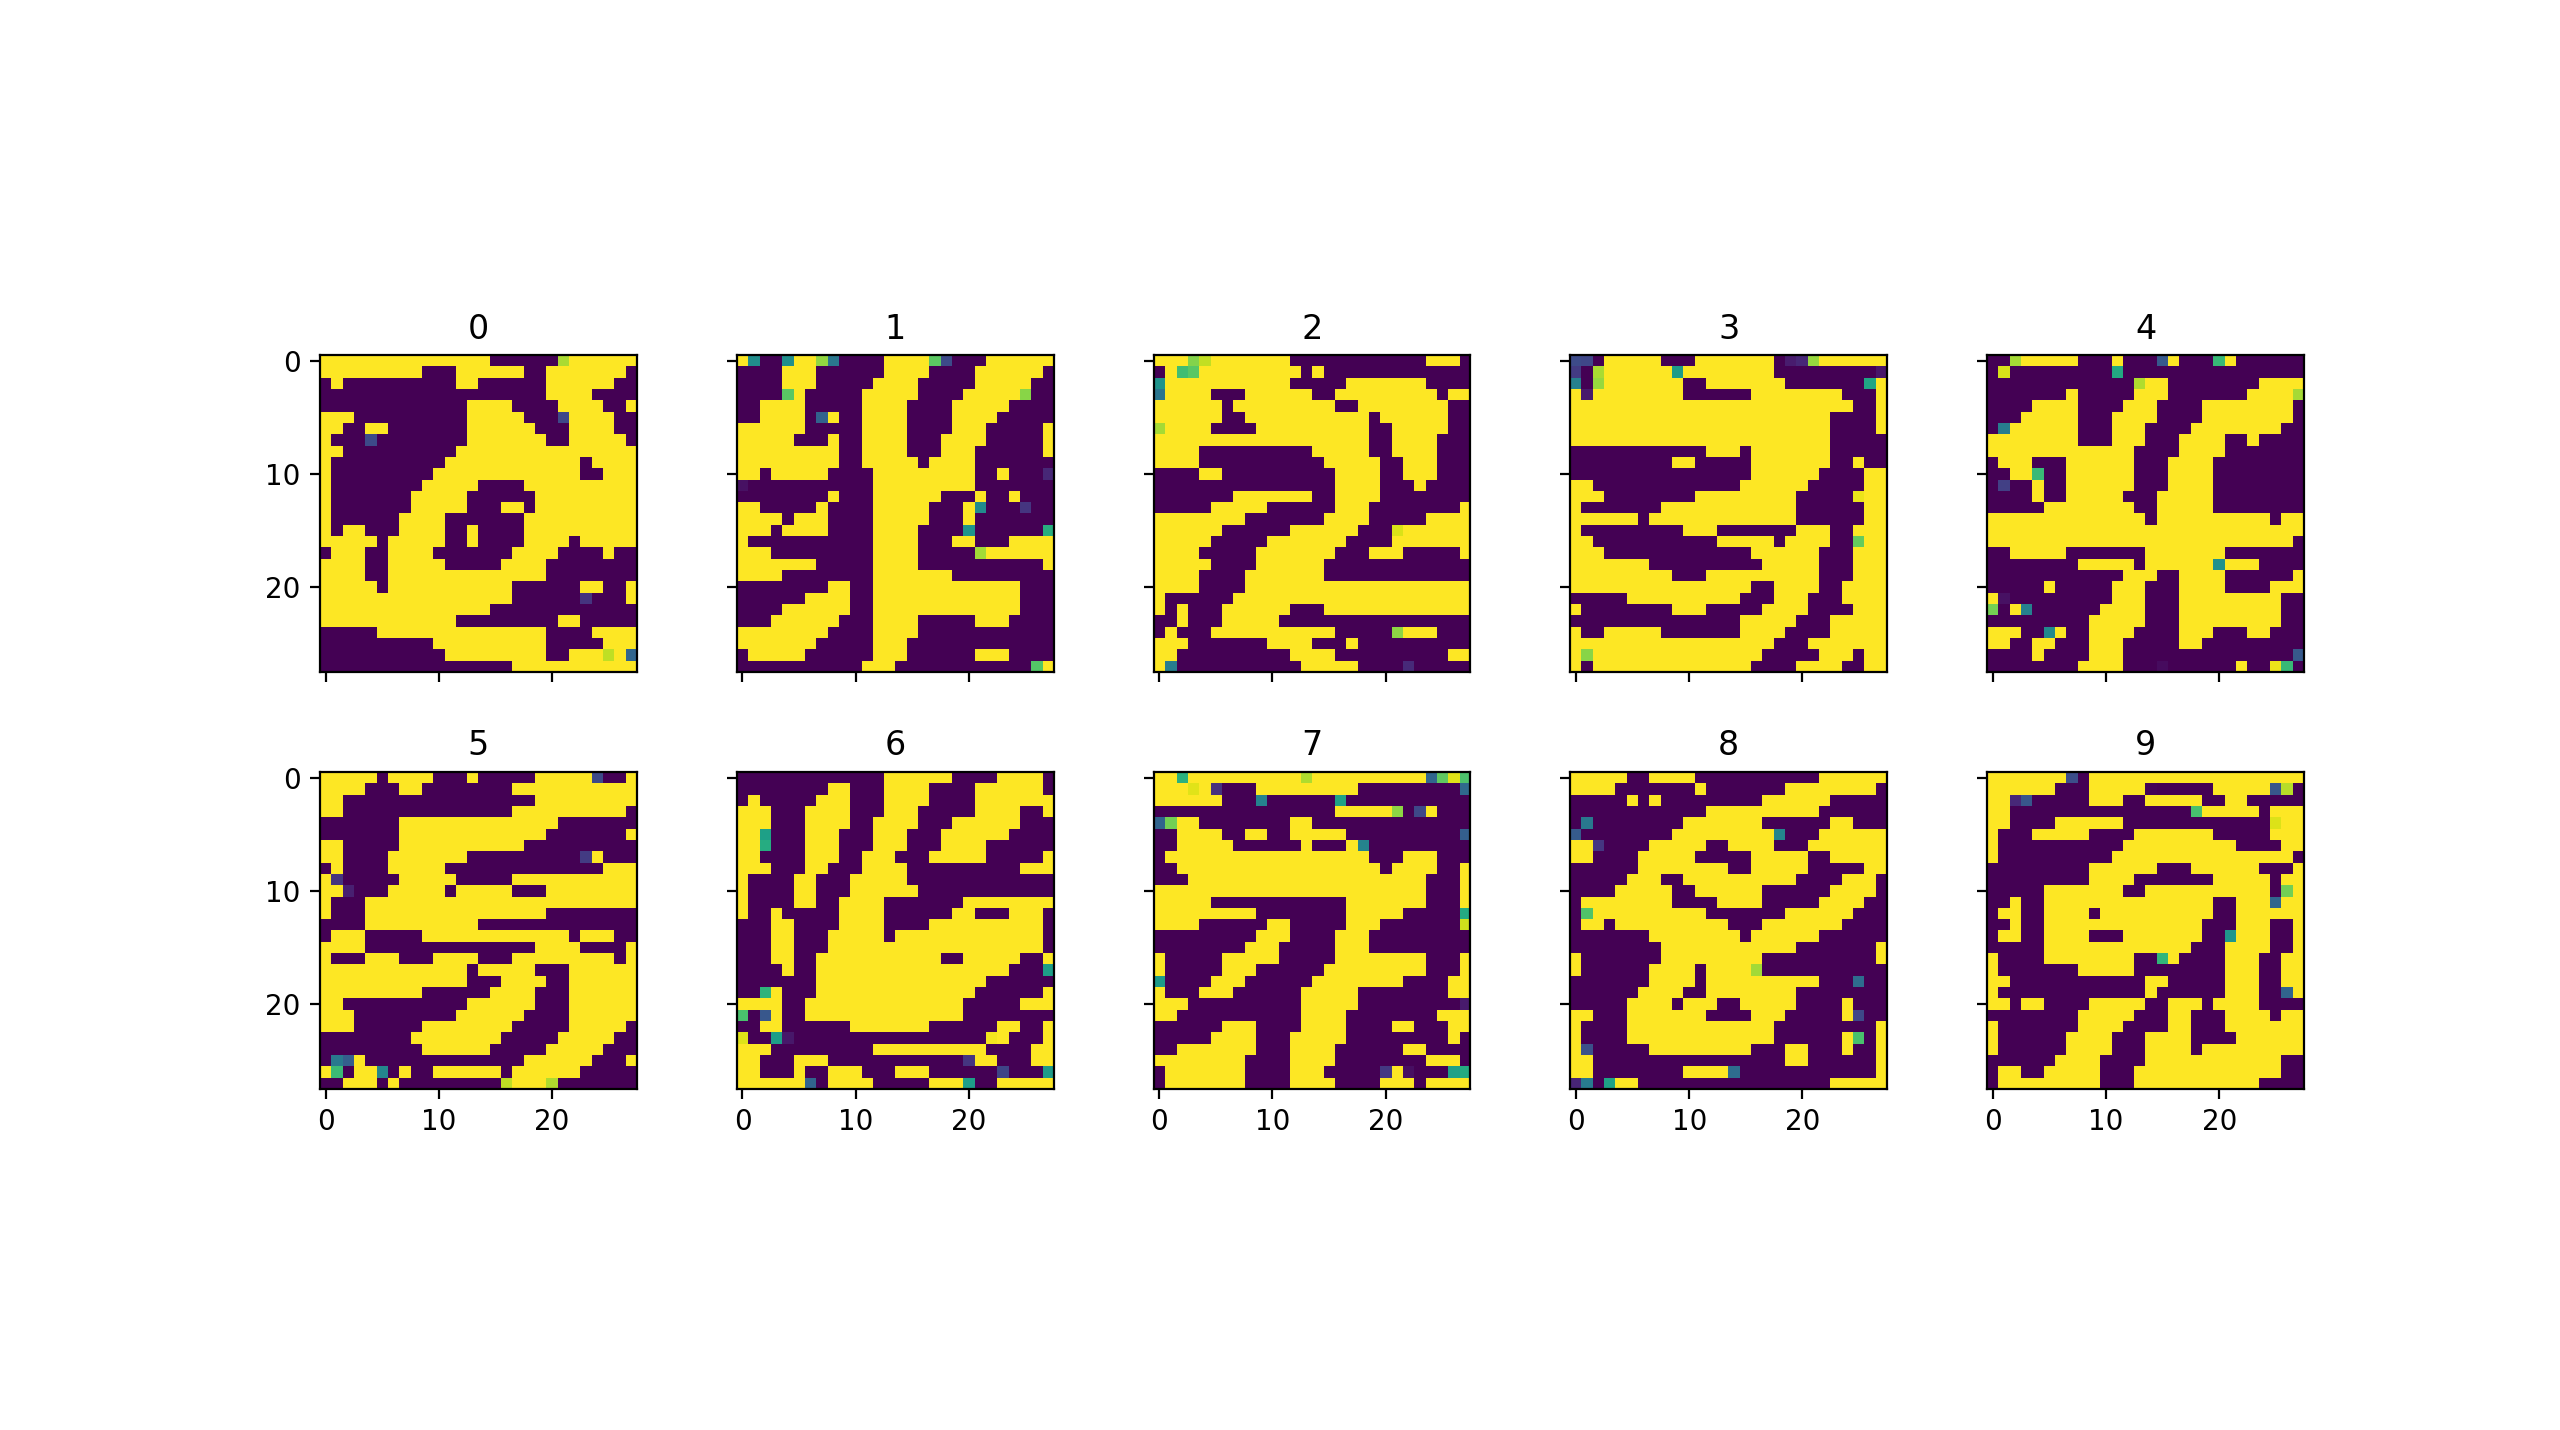
\includegraphics[scale=0.57]{q3_last_layer}
\end{center}

\subsection{Plot of $x_{init}$ for 10 Feature Maps after $2^{nd}$ Max Pooling}
\begin{center}
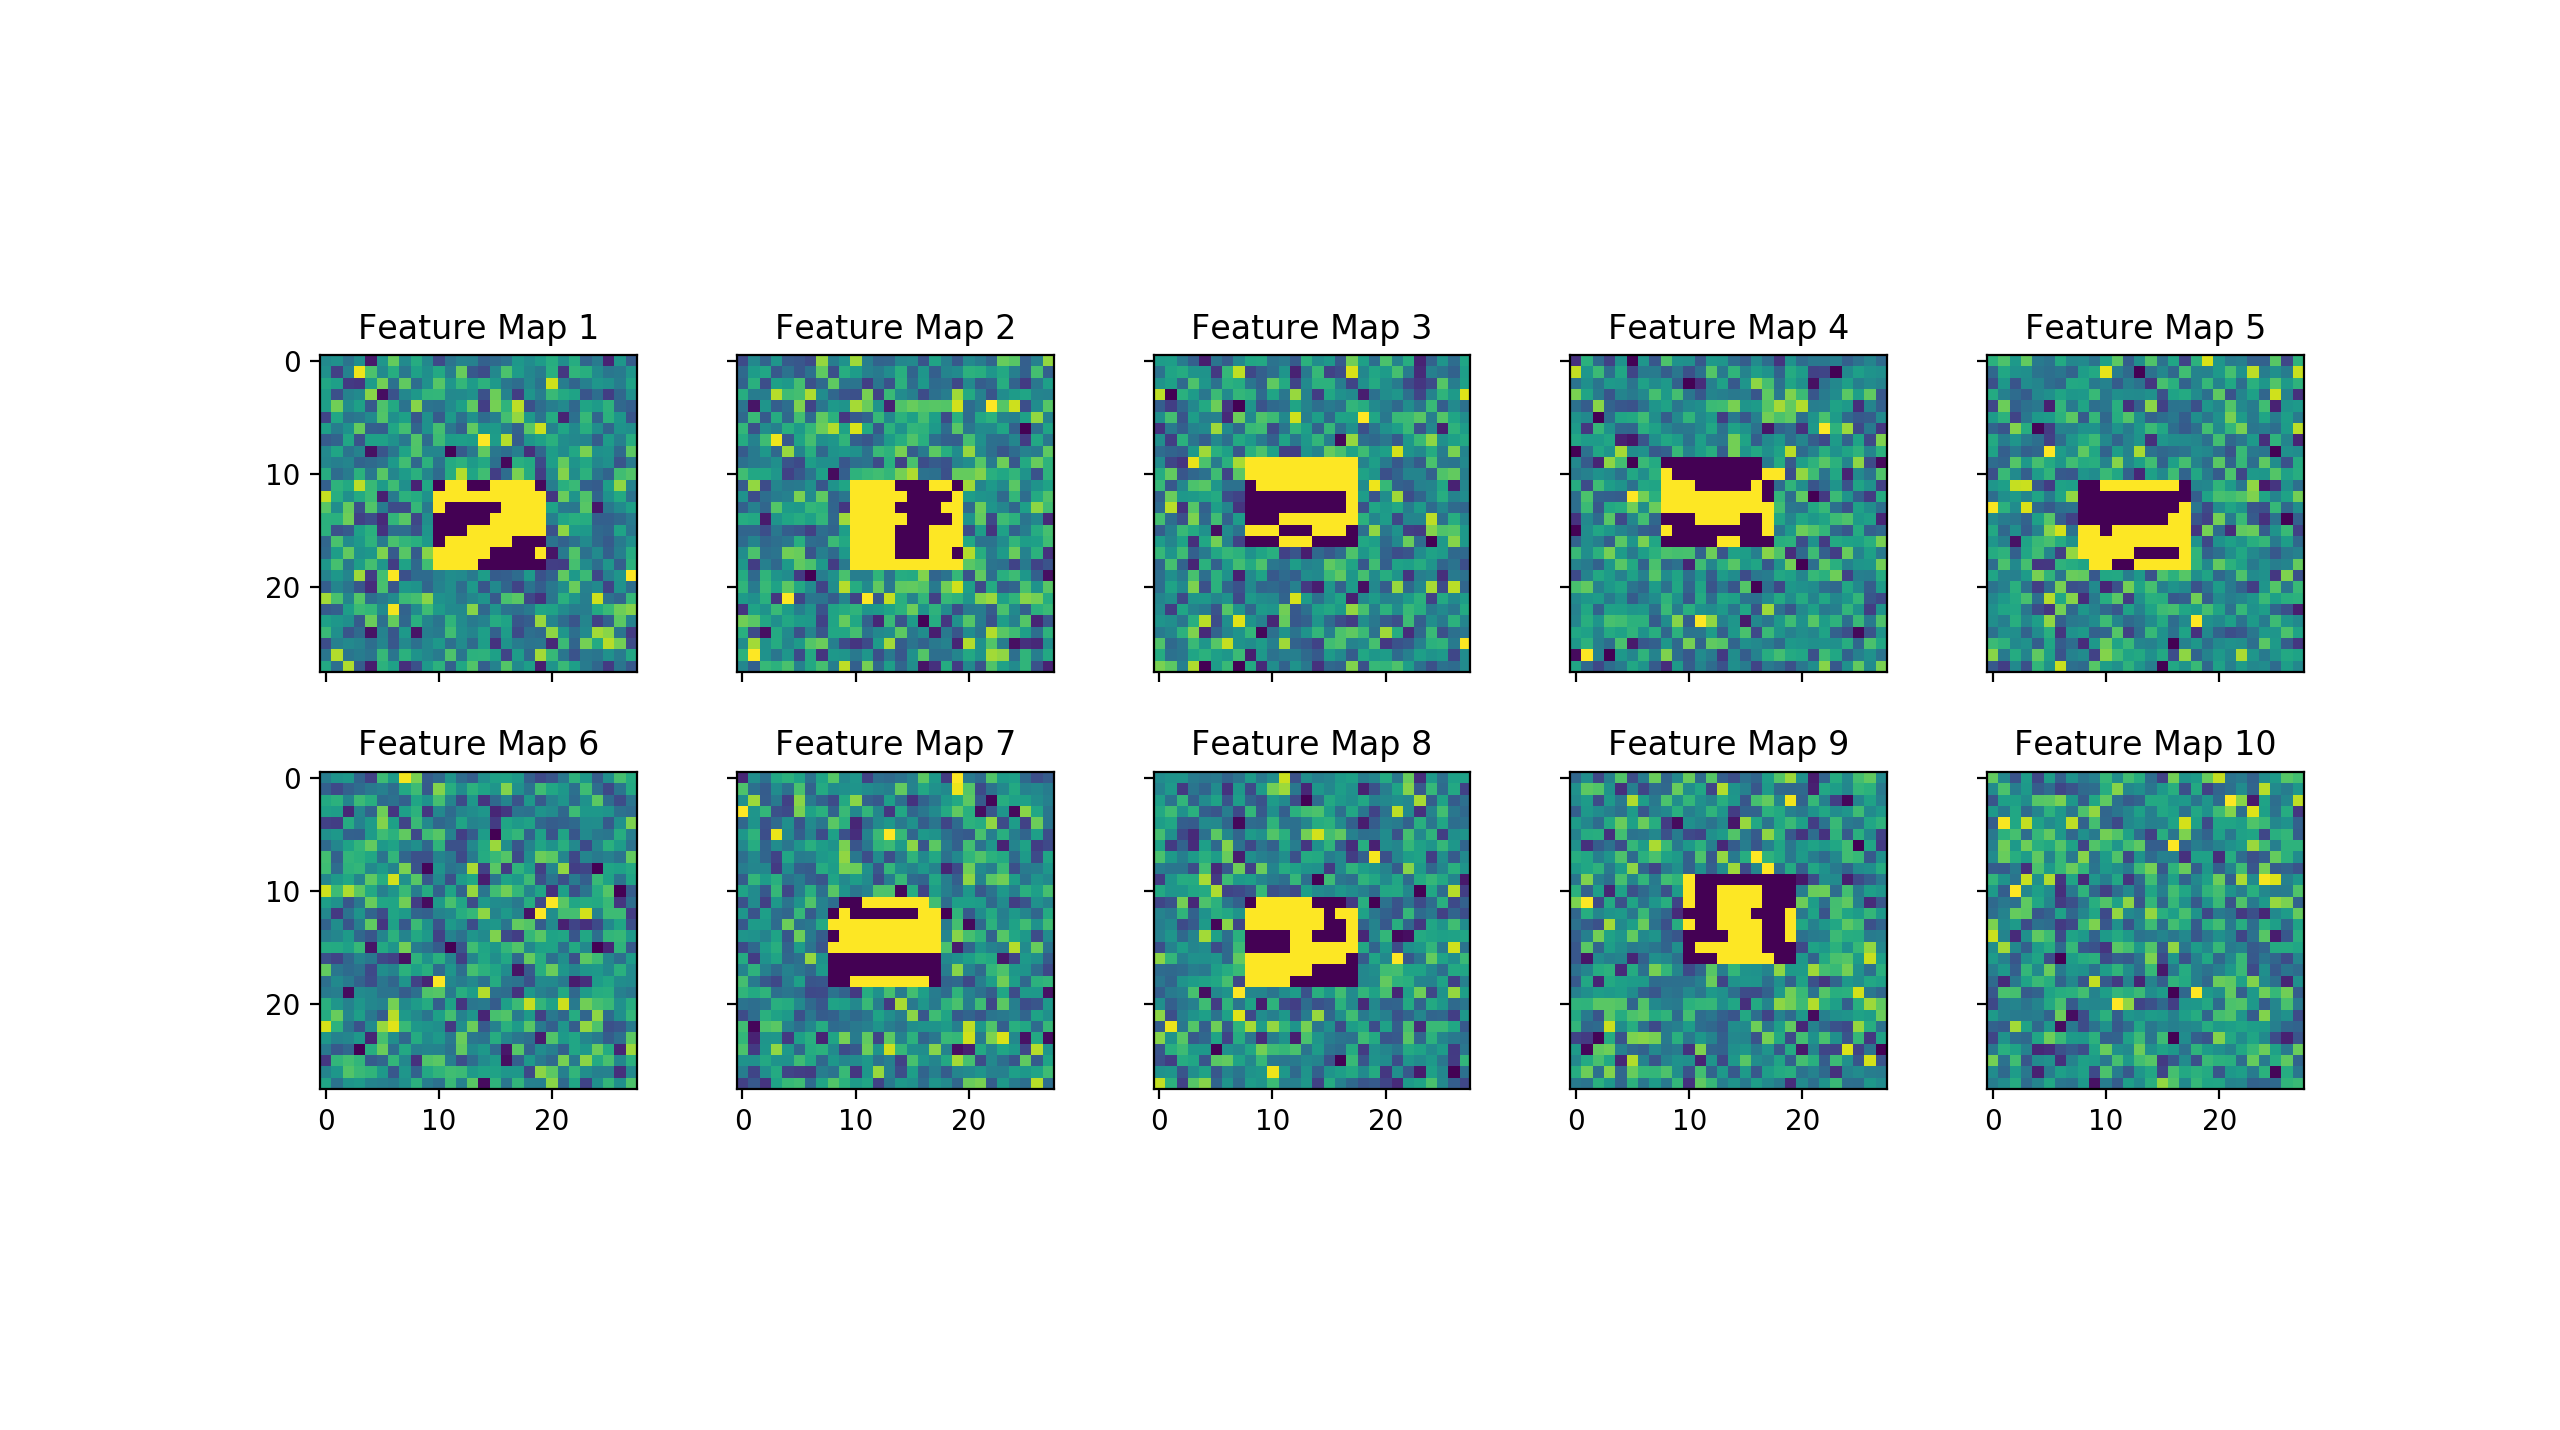
\includegraphics[scale=0.57]{Figure_2}
\end{center}

\end{document}
